\documentclass[12pt, oneside, final]{report}
\usepackage{geometry}
\geometry{a4paper, left=20mm, right=20mm, top=25mm, bottom=25mm}
\usepackage[utf8]{inputenc}
\usepackage{t1enc}
\usepackage[MeX]{polski}
\usepackage{graphicx}
\usepackage{amsmath}
\usepackage{amssymb}
\usepackage{mathtools}
\usepackage{indentfirst}
\usepackage{pdfpages}
\usepackage{xcolor}
\usepackage{placeins} % provides \FloatBarrier
\usepackage{tikz}
\usetikzlibrary{positioning,shapes,arrows,calc,decorations.markings,shadows}
\usepackage[hidelinks]{hyperref}

% Czcionka
\usepackage{charter}

% Pojedyncze elementy na górze stron
\makeatletter
\setlength{\@fptop}{0pt}
\makeatother

% Styl tytułowania rozdziałów:
\usepackage{titlesec}
%\titleformat{\chapter}{\normalfont\huge}{\bf\thechapter.}{20pt}{\huge\bf}
% Styl tytułowania rozdziałów:
\titleformat{\chapter}[display] 
{\centering\normalfont\huge\bfseries}{\centering\chaptertitlename\ \thechapter.}{0.5em}{}
\titlespacing{\chapter}{0em}{0em}{2em}

% dodatkowe kropki po numerach rozdziałów, sekcji itd
\usepackage{titlesec}
\titlelabel{\thetitle.\quad}

% Dodatkowe odstępy w tabelach
\usepackage{array}
\setlength\extrarowheight{4pt}

% Wyłączone wcięcia
\usepackage{parskip}

% tabucline
\usepackage{tabu}

\definecolor{fed}{RGB}{71,47,145}
\definecolor{ex}{RGB}{245,121,33}

\begin{document}
% Title page
\begin{titlepage}
	\centering
	\begin{figure}
		\centering
		
\includegraphics[width=0.9\textwidth]{logo.pdf}
	\end{figure}
	\vspace*{100pt}
	\LARGE{Przetwarzanie cyfrowe obrazów}\\
	\vspace{30pt}
	\textsc{\Huge{Rozpoznawanie logo FedEx}}\\
	\vspace{10pt}
	\large{Sprawozdanie z projektu}\\
	\vspace{120pt}
	\Large{Łukasz Kilaszewski \textit{259822}}\\
	\vfill
	\large{23 stycznia 2018}
\end{titlepage}

\thispagestyle{empty}
%\tableofcontents
%\cleardoublepage

\section*{Wstęp}
Podstawowym celem projektu było napisanie aplikacji, która będzie w stanie rozpoznać fragmenty "Fed" oraz "Ex" z logo firmy FedEx. logo to przedstawione zostało na poniższym rysunku.
\begin{figure}[ht!]
	\centering
	
\includegraphics[width=0.4\textwidth]{images/logo.jpg}
	\caption{Logo firmy FedEx.}
\end{figure}

W przedstawionym logo można wyróżnić dwa kolory podstawowe, które jednoznacznie identyfikują jego części. Ten fakt stanowił podstawę do implementacji algorytmu segmentacji.

\section*{Etapy przetwarzania obrazu}
\subsection*{Przygotowanie obrazu}
Obraz po wczytaniu jest konwertowany do przestrzeni barw HSV. Pozwala to wydzielić barwę (ang. \textit{hue}), nasycenie(ang. \textit{saturation}) oraz jasność (wartość - ang. \textit{value}). Przyjęte wartości składowych każdego piksela to liczby całkowite z zakresów:
\begin{figure}[ht!]
	\centering
	\begin{tabular}{|l|c|c|}
		\hline
		Skłądowa & Wartość min. & Wartość max.\\
		\hline
		Hue & 0 & 179\\
		Saturation & 0 & 255\\
		Value & 0 & 255\\
		\hline
	\end{tabular}
\end{figure}

W trakcie realizacji projektu, w celu usunięcia szumów z obrazów, zastosowana została filtracja dolnoprzepustowa za pomocą filtra konwolucyjnego i jednej z następujących macierzy:
$$ 
\mathbf{F_1} = 
\left[\begin{matrix}
\frac{1}{9} & \frac{1}{9} & \frac{1}{9}\\
\frac{1}{9} & \frac{1}{9} & \frac{1}{9}\\
\frac{1}{9} & \frac{1}{9} & \frac{1}{9}
\end{matrix}\right]
$$
$$
\mathbf{F_2} = 
\left[\begin{matrix}
\frac{1}{25} & \frac{1}{25} & \frac{1}{25} & \frac{1}{25} & \frac{1}{25}\\
\frac{1}{25} & \frac{1}{25} & \frac{1}{25} & \frac{1}{25} & \frac{1}{25}\\
\frac{1}{25} & \frac{1}{25} & \frac{1}{25} & \frac{1}{25} & \frac{1}{25}\\
\frac{1}{25} & \frac{1}{25} & \frac{1}{25} & \frac{1}{25} & \frac{1}{25}\\
\frac{1}{25} & \frac{1}{25} & \frac{1}{25} & \frac{1}{25} & \frac{1}{25}
\end{matrix}\right]
$$

Operacja ta nie przynosiła jednak zauważalnej poprawy w jakości segmentacji i klasyfikacji, dlatego została usunięta.

\subsection*{Segmentacja}
Zgodnie z wcześniejszą obserwacją, elementy rozpoznawanego logo różnią się barwą, dlatego ich segmentacja oparta jest o prosty algorytm, działający na obrazie wejściowym w przestrzeni barw HSV. Z obrazu wydzielane są dwie grupy pikseli. Warunki przynależności piksela \texttt{p} o składowych \texttt{p.H}, \texttt{p.S}, \texttt{p.V} do jednej z grup to:

Grupa "Fed": \texttt{(p.H >= FED\_H\_VAL - FED\_H\_EPS) \&\& (p.H <= FED\_H\_VAL + FED\_H\_EPS) \&\& (p.S >= FED\_S\_MIN)}

Grupa "Ex": \texttt{(p.H >= EX\_H\_VAL - EX\_H\_EPS) \&\& (p.H <= EX\_H\_VAL + EX\_H\_EPS) \&\& (p.S >= EX\_S\_MIN)}

Wartości stałych \texttt{FED\_H\_VAL} oraz \texttt{EX\_H\_VAL} zostały odczytane z obrazu przedstawiającego logo za pomocą programu do obróbki obrazów rastrowych. Pozostałe stałe zostały dobrane w sposób eksperymentalny. Wartości stałych wynoszą odpowiednio:
\begin{figure}[ht!]
	\centering
	\begin{tabular}{|l|l|}
		\hline
		Stała & Wartość\\
		\hline
		FED\_H\_VAL & 122\\
		FED\_H\_EPS & 10\\
		FED\_S\_MIN & 100\\
		EX\_H\_VAL & 5\\
		EX\_H\_EPS & 10\\
		EX\_S\_MIN & 100\\
		\hline
	\end{tabular}
\end{figure}

Wynikiem segmentacji są dwie mapy bitowe przedstawiające przynależność pikseli do danej grupy.

Kolejnym etapem jest filtracja otrzymanych map bitowych. W tym celu najpierw obie mapy są zamykane za pomocą dylatacji (macierz 5 $\times$ 5) i erozji (macierz 3 $\times$ 3).

Następnie z otrzymanych map ekstrahowane są obiekty, które mogą być rozpoznawanymi elementami logo. W tym celu używany jest algorytm zalewania (ang. \textit{flood fill}), który grupuje sąsiadujące ze sobą piksele. Obiekty złożone z mniej niż \texttt{SEGMENT\_MIN\_PIXELS = 150} pikseli są odrzucane, ponieważ nie mogą zawierać w sobie elementu logo i stanowią szum. Wartość tego parametru dobrana została w sposób eksperymentalny.

\subsection*{Klasyfikacja}
Po segmentacji otrzymujemy zbiór grup pikseli (obiektów), które są domniemanymi elementami rozpoznawanego logo. Należy odrzucić te grupy, które nie zostały rozpoznane jako interesujące. W tym celu zastosowane są współczynniki kształtu i momenty geometryczne. W celu wybrania tych parametrów, które pozwolą na rozpoznawanie elementów logo, przeprowadzono eksperyment na specjalnie przygotowanym obrazie testowym. Wyniki segmentacji tego obrazu przedstawiono na rysunku \ref{test}.

\begin{figure}[ht!]
	\centering
	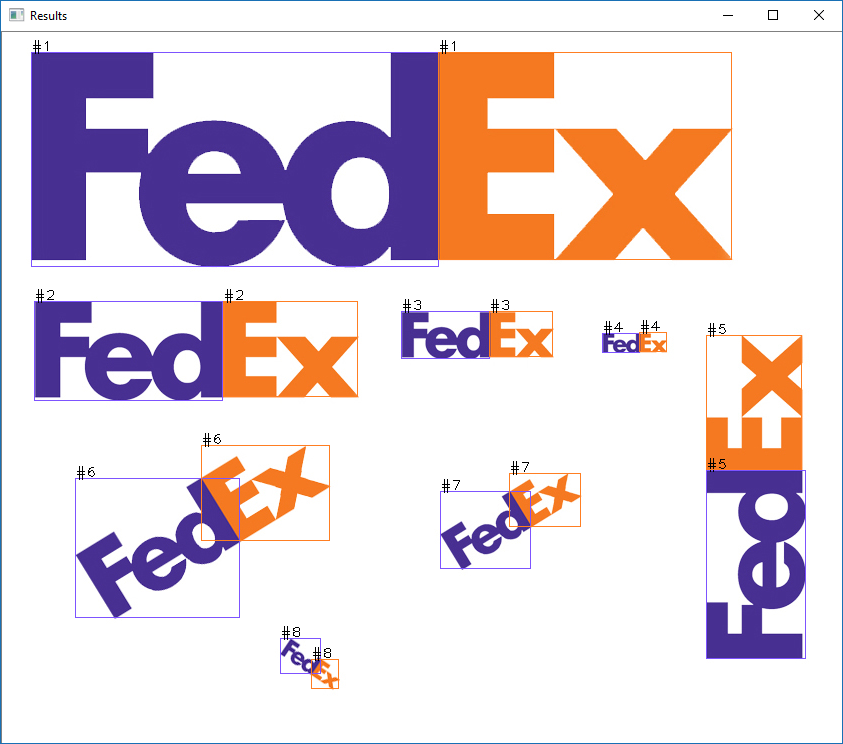
\includegraphics[width=\textwidth]{images/test_image.png}
	\caption{Wynik działania segmentacji dla obrazu testowego.}
	\label{test}
\end{figure}

Dla każdego z segmentów wyznaczono wartości pewnych parametrów. Otrzymane wyniki przedstawione zostały w tabeli \ref{params}.

\begin{table}[ht!]
	\footnotesize
	\begin{tabu}{|l|l|l|l|l|l|l|l|l|}
		\hline
		Segment & W3 & W6 & M1 & M2 & M3 & M4 & M6 & M7\\
		\hline
		\textcolor{fed}{\#1} & 2.220393 & 0.902794 & 0.385664 & 0.072226 & 0.001927 & 0.000550 & -0.000068 & 0.019128\\
		\textcolor{fed}{\#2} & 2.040321 & 0.903828 & 0.364132 & 0.063494 & 0.001624 & 0.000460 & -0.000055 & 0.017275\\
		\textcolor{fed}{\#3} & 1.633803 & 0.915984 & 0.328471 & 0.050386 & 0.001184 & 0.000333 & -0.000040 & 0.014377\\
		\textcolor{fed}{\#4} & 0.656992 & 0.941814 & 0.272966 & 0.033802 & 0.000508 & 0.000162 & -0.000012 & 0.010177\\
		\textcolor{fed}{\#5} & 2.040576 & 0.904119 & 0.364710 & 0.063649 & 0.001659 & 0.000165 & -0.000067 & 0.017341\\
		\textcolor{fed}{\#6} & 2.378524 & 0.910247 & 0.351664 & 0.058832 & 0.001419 & 0.000628 & -0.000046 & 0.016209\\
		\textcolor{fed}{\#7} & 1.808266 & 0.936040 & 0.317345 & 0.046307 & 0.001177 & 0.000532 & -0.000034 & 0.013600\\
		\textcolor{fed}{\#8} & 0.799410 & 0.941694 & 0.268004 & 0.032672 & 0.000673 & 0.000206 & -0.000011 & 0.009788\\
		\hline
		ŚREDNIA & 1.697286 & 0.924277 & 0.331620 & 0.052671 & 0.001271 & 0.000380 & -0.000042 & 0.014737\\
		\hline
		MIN & 0.656992 & 0.902794 & 0.268004 & 0.032672 & 0.000508 & 0.000162 & -0.000068 & 0.009788\\
		\hline
		MAX & 2.378524 & 0.941814 & 0.385664 & 0.072226 & 0.001927 & 0.000628 & -0.000011 & 0.019128\\\tabucline[2pt]{-}
		\textcolor{ex}{\#1} & 1.807662 & 0.915587 & 0.305149 & 0.018762 & 0.005164 & 0.001851 & 0.000032 & 0.018588\\
		\textcolor{ex}{\#2} & 1.639025 & 0.915780 & 0.288693 & 0.016731 & 0.004153 & 0.001466 & 0.000021 & 0.016653\\
		\textcolor{ex}{\#3} & 1.352058 & 0.915034 & 0.265987 & 0.014446 & 0.003175 & 0.001103 & 0.000013 & 0.014076\\
		\textcolor{ex}{\#4} & 0.309014 & 0.965764 & 0.202308 & 0.009096 & 0.001064 & 0.000408 & 0.000006 & 0.007958\\
		\textcolor{ex}{\#5} & 1.661269 & 0.916043 & 0.289890 & 0.016688 & 0.004158 & 0.000469 & 0.000017 & 0.016837\\
		\textcolor{ex}{\#6} & 1.926532 & 0.917138 & 0.273685 & 0.013799 & 0.003590 & 0.000404 & 0.000021 & 0.015276\\
		\textcolor{ex}{\#7} & 1.574777 & 0.921030 & 0.245667 & 0.010118 & 0.002552 & 0.000274 & 0.000013 & 0.012558\\
		\textcolor{ex}{\#8} & 0.723016 & 0.941940 & 0.197575 & 0.005540 & 0.001118 & 0.000044 & 0.000003 & 0.008374\\
		\hline
		ŚREDNIA & 1.374169 & 0.926040 & 0.258619 & 0.013148 & 0.003122 & 0.000752 & 0.000016 & 0.013790\\
		\hline
		MIN & 0.309014 & 0.915034 & 0.197575 & 0.005540 & 0.001064 & 0.000044 & 0.000003 & 0.007958\\
		\hline
		MAX & 1.926532 & 0.965764 & 0.305149 & 0.018762 & 0.005164 & 0.001851 & 0.000032 & 0.018588\\
		\hline
	\end{tabu}
	\caption{Wartości wyznaczonych parametrów dla segmentów z obrazu testowego.}
	\label{params}
\end{table}

Zdecydowano, że do rozpoznawania elementu "Fed" wykorzystane zostaną parametry W6, M1, M2, M7. Ten sam zbiór parametrów początkowo wykorzystywany był do rozpoznawania elementu "Ex", natomiast w trakcie eksperymentów zdecydowano, że konieczne jest dodanie jeszcze jednego warunku. Zbiór parametrów wykorzystywanych do klasyfikacji elementów "Ex" to: W6, M1, M2, M6, M7.

Klasyfikacja polega na sprawdzeniu, czy wszystkie parametry elementu mieszczą się w odpowiednich zakresach. Wartości maksymalne i minimalne dobrano na podstawie tabeli \ref{test} oraz eksperymentów. Są one opisane przez stałe zestawione w tabeli \ref{consts}.
\begin{figure}[ht!]
	\centering
	\begin{tabular}{|l|l|}
		\hline
		Stała & Wartość\\
		\hline
		\texttt{FED\_W6\_MIN} & 0.902\\
		\texttt{FED\_W6\_MAX} & 0.944\\
		\texttt{FED\_M1\_MIN} & 0.267\\
		\texttt{FED\_M1\_MAX} & 0.397\\
		\texttt{FED\_M2\_MIN} & 0.032\\
		\texttt{FED\_M2\_MAX} & 0.082\\
		\texttt{FED\_M7\_MIN} & 0.009\\
		\texttt{FED\_M7\_MAX} & 0.020\\
		\texttt{EX\_W6\_MIN} & 0.914\\
		\texttt{EX\_W6\_MAX} & 0.966\\
		\texttt{EX\_M1\_MIN} & 0.197\\
		\texttt{EX\_M1\_MAX} & 0.306\\
		\texttt{EX\_M2\_MIN} & 0.005\\
		\texttt{EX\_M2\_MAX} & 0.022\\
		\texttt{EX\_M6\_MIN} & 0.000002\\
		\texttt{EX\_M6\_MAX} & 0.000036\\
		\texttt{EX\_M7\_MIN} & 0.007\\
		\texttt{EX\_M7\_MAX} & 0.019\\
		\hline
	\end{tabular}
	\caption{Stałe definiujące zakresy wartości parametrów.}
	\label{consts}
\end{figure}

\section*{Grupowanie}
Po klasyfikacji elementy stanowiące jedno logo łączone są w pary, a następnie rysowane są prostokąty obejmujące całe logo (ang. \textit{bounding box}). Algorytm łączący w pary wyznacza dla każdego z elementów 8 punktów charakterystycznych:
\begin{itemize}
	\item lewy górny róg prostokąta ograniczającego,
	\item lewy dolny róg prostokąta ograniczającego,
	\item prawy dolny róg prostokąta ograniczającego,
	\item prawy górny róg prostokąta ograniczającego,
	\item punkt wspólny elementu i lewej krawędzi prostokąta ograniczającego,
	\item punkt wspólny elementu i dolnej krawędzi prostokąta ograniczającego,
	\item punkt wspólny elementu i prawej krawędzi prostokąta ograniczającego,
	\item punkt wspólny elementu i górnej krawędzi prostokąta ograniczającego.
\end{itemize}
Elementy, których zbiory punktów mają co najmniej 2 pary punktów odległych o nie więcej niż \texttt{GROUP\_MAX\_DIST = 8} stanowią jedno logo. Wartość stałej \texttt{GROUP\_MAX\_DIST} dobrana została na drodze eksperymentów.

\section*{Wyniki}
Poniżej przedstawiono wyniki działania programu dla różnych obrazów wejściowych. Program z zadowalającą skutecznością rozpoznaje logo firmy FedEx na obrazach.

Na rysunku 7. - zgodnie z oczekiwaniami - nie został rozpoznany element "Fed" w białym kolorze.

Program nie rozpoznał również jednego z elementów "Ex" na rysunku 8. Prawdopodobnie spowodowane jest to faktem, że element ten jest zniekształcony ze względu na perspektywę.
\begin{figure}[ht!]
	\centering
	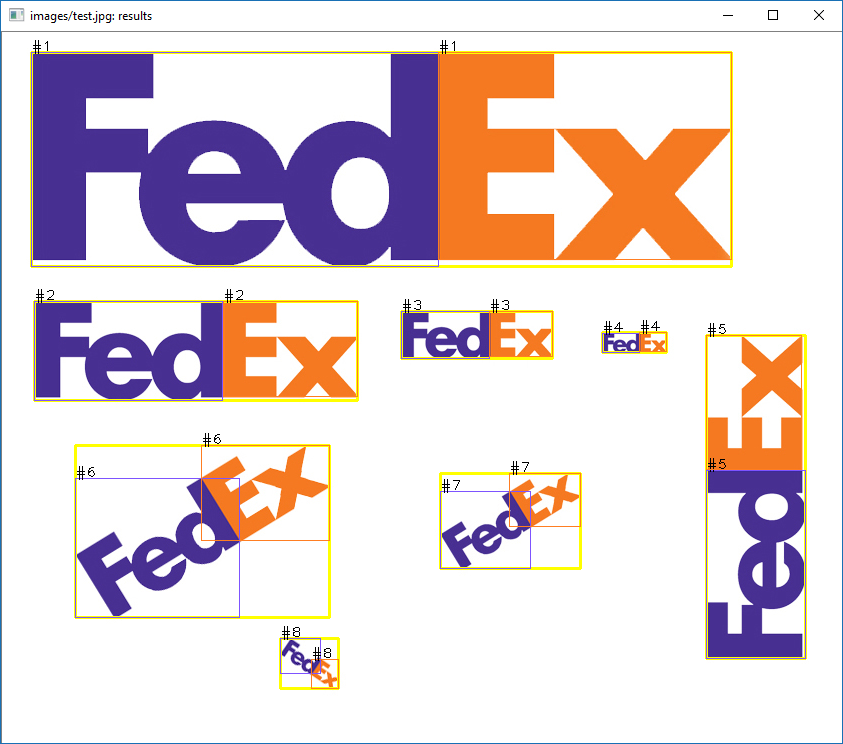
\includegraphics[height=0.4\textheight]{images/result0.png}
	\caption{Wynik działania programu dla obrazu testowego.}
\end{figure}
\begin{figure}[ht!]
	\centering
	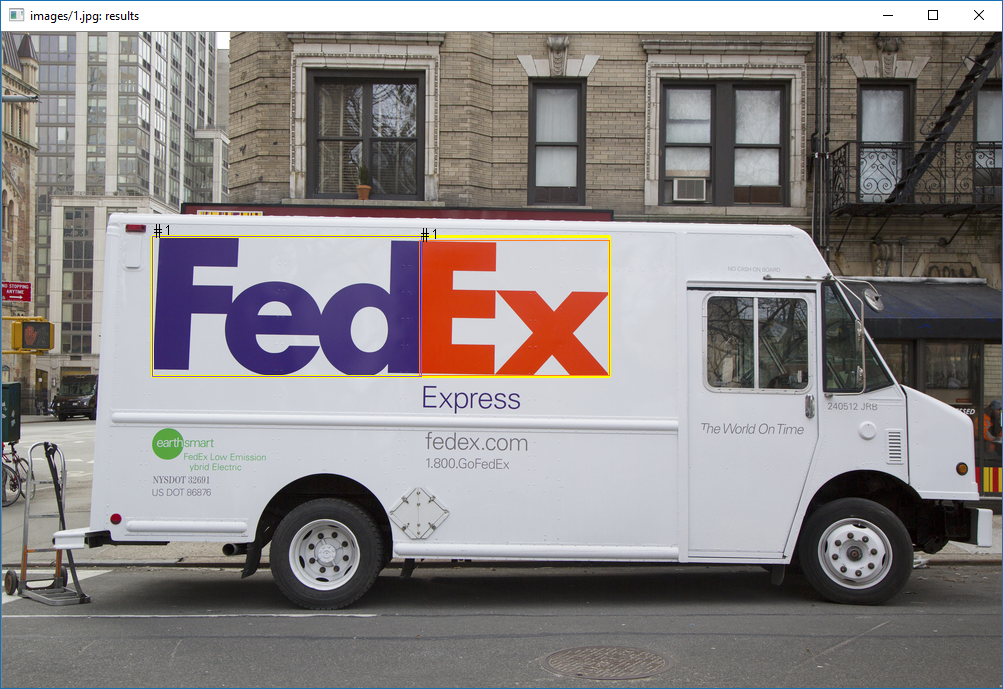
\includegraphics[height=0.4\textheight]{images/result1.png}
	\caption{Wynik działania programu dla obrazu \textit{images/1.jpg}.}
\end{figure}
\begin{figure}[ht!]
	\centering
	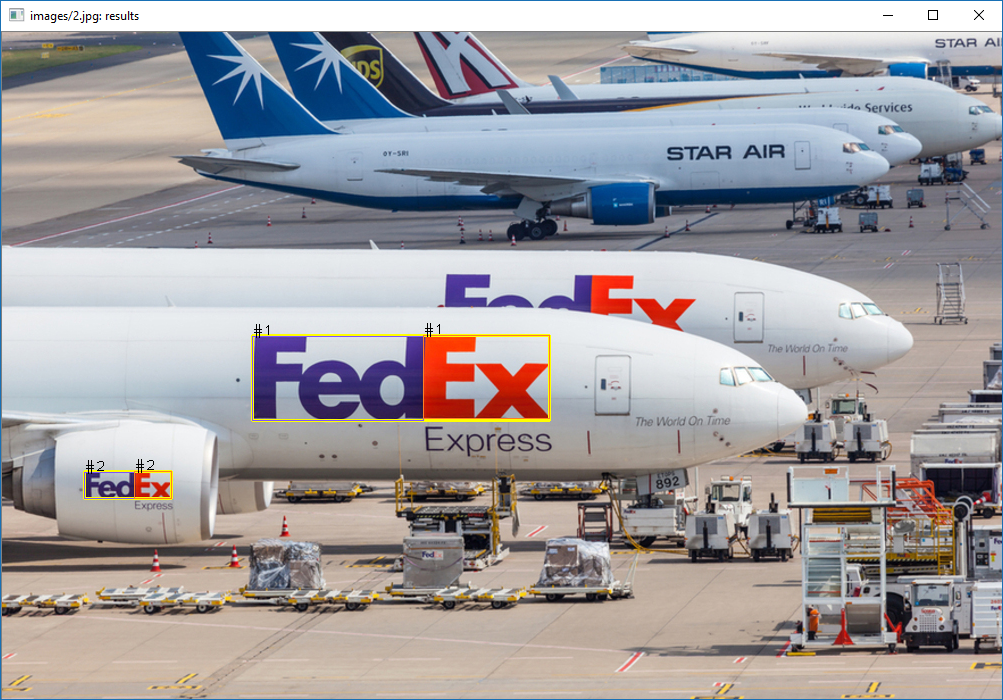
\includegraphics[height=0.4\textheight]{images/result2.png}
	\caption{Wynik działania programu dla obrazu \textit{images/2.jpg}.}
\end{figure}
\begin{figure}[ht!]
	\centering
	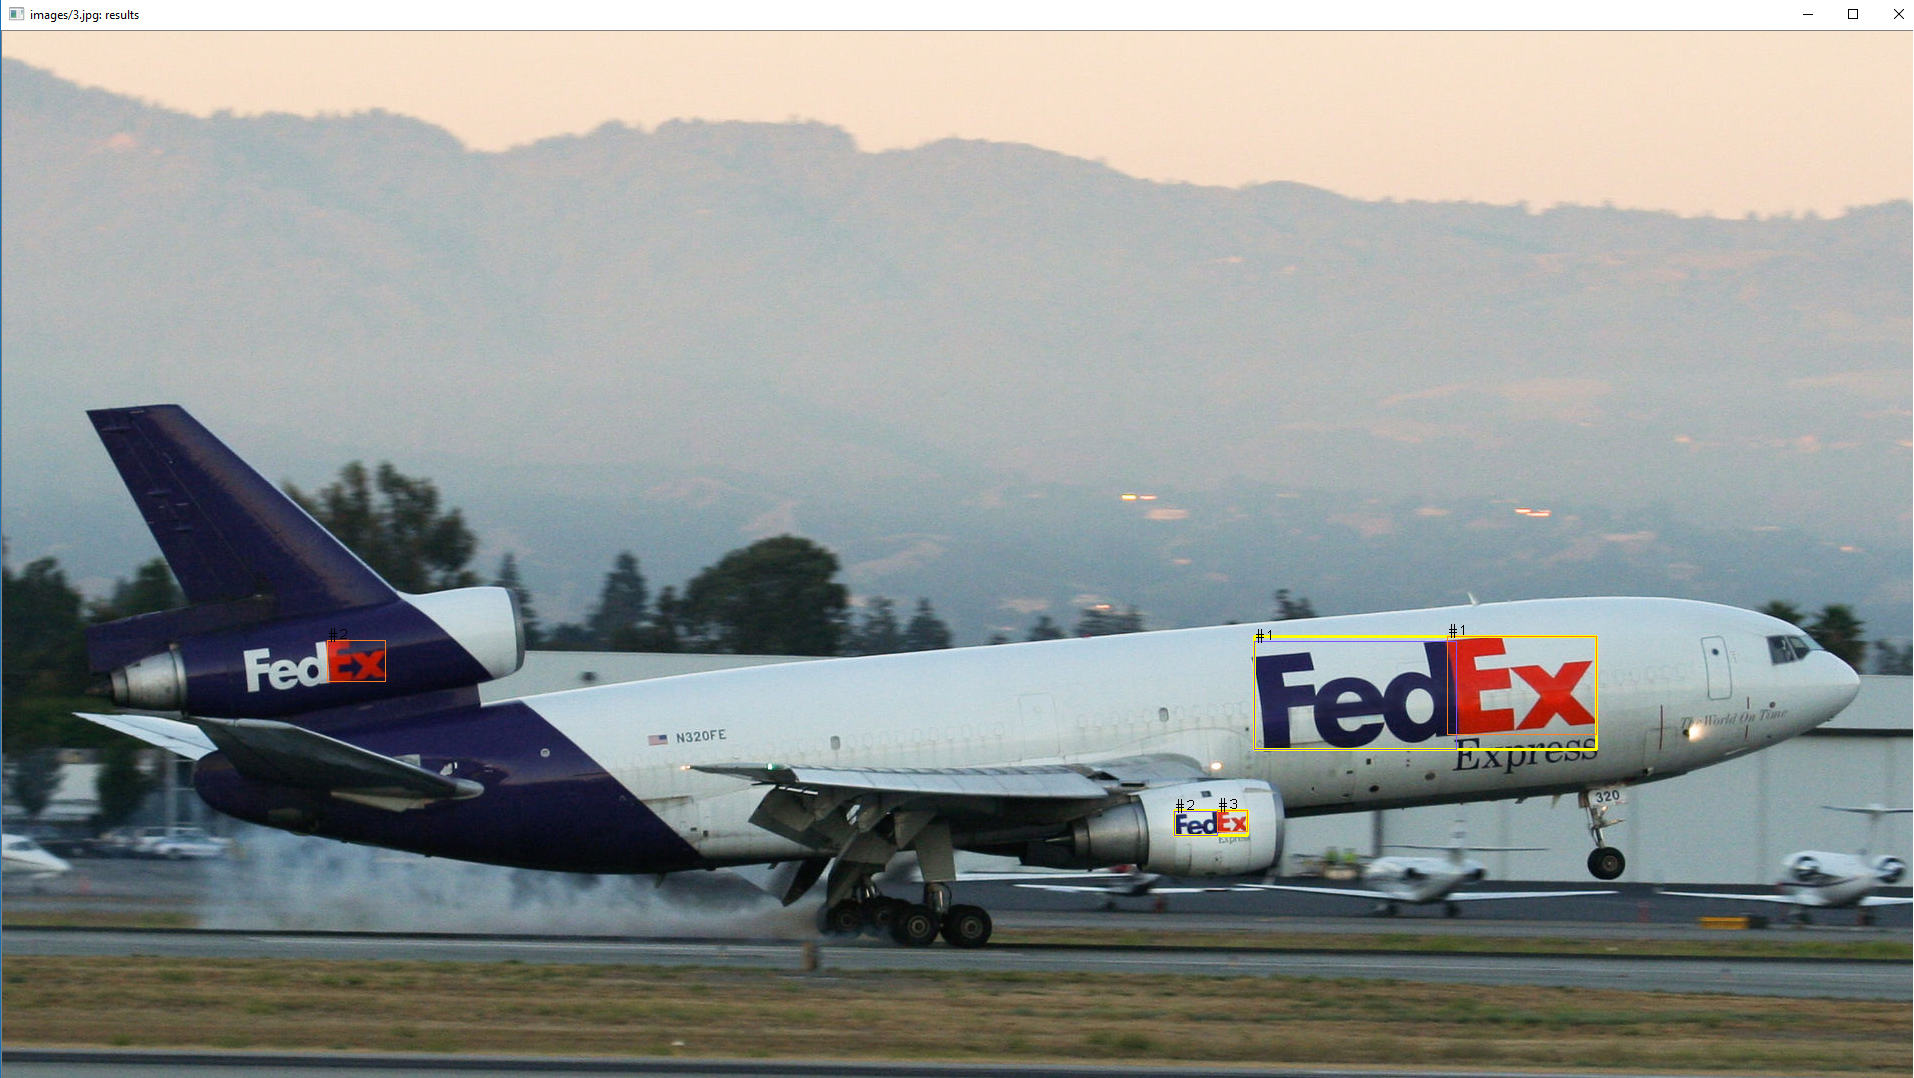
\includegraphics[height=0.4\textheight]{images/result3.png}
	\caption{Wynik działania programu dla obrazu \textit{images/3.jpg}.}
\end{figure}
\begin{figure}[ht!]
	\centering
	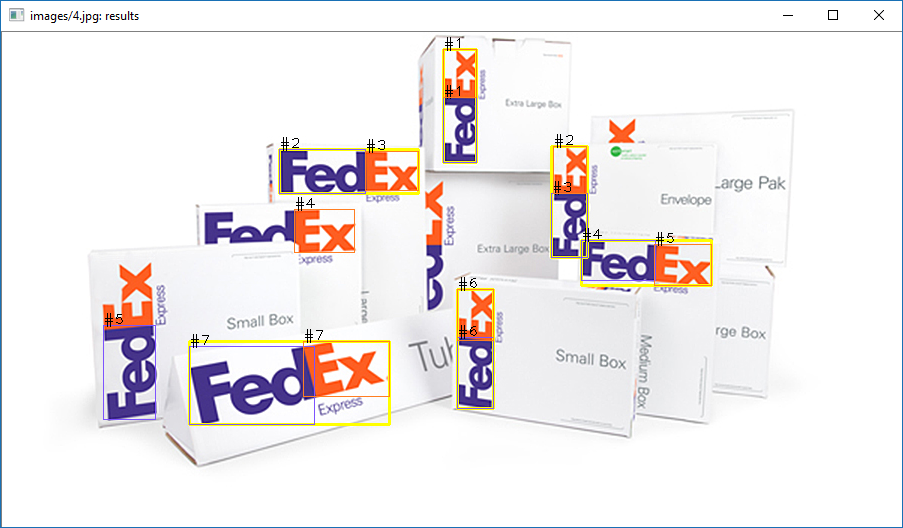
\includegraphics[height=0.4\textheight]{images/result4.png}
	\caption{Wynik działania programu dla obrazu \textit{images/4.jpg}.}
\end{figure}


\end{document}
